% Auto-generated by generate_report.py — do not edit manually
% Cream-background slide variant — same content as the report version with
% canvabg pagecolor for use against the presentation theme.
\documentclass[border=8pt]{standalone}
\usepackage{fontspec}
\setmainfont{Carlito}
\usepackage{unicode-math}
\setmathfont{Latin Modern Math}
\usepackage{xcolor}
\usepackage{pgfplots}
\pgfplotsset{compat=1.18}
\usepgfplotslibrary{groupplots}
\usetikzlibrary{patterns,positioning}
\definecolor{canvabg}{RGB}{246,244,241}
\pagecolor{canvabg}
\begin{document}
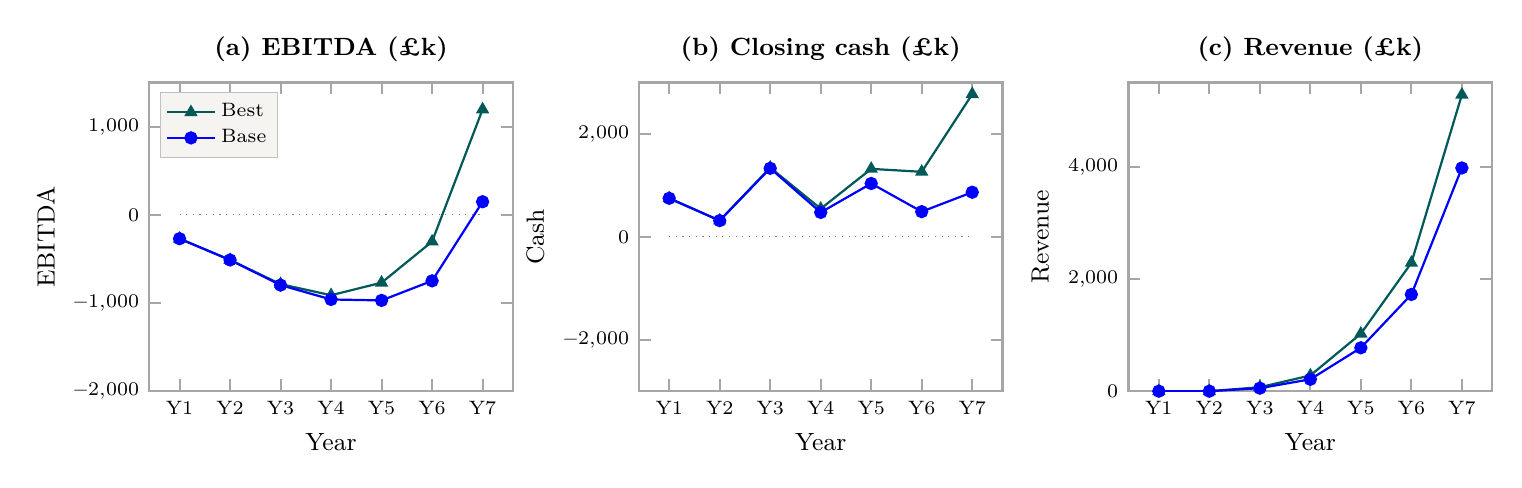
\begin{tikzpicture}
    \begin{groupplot}[
        group style={
            group size=3 by 1,
            horizontal sep=1.6cm,
        },
        width=6.2cm,
        height=5.5cm,
        symbolic x coords={Y1,Y2,Y3,Y4,Y5,Y6,Y7},
        xtick=data,
        xlabel={Year},
        axis line style={line width=0.9pt, draw=gray!70},
        tick style={line width=0.7pt, color=gray!70},
        tick label style={font=\scriptsize},
        label style={font=\small},
        title style={font=\small\bfseries, yshift=-2pt},
        legend style={
            font=\scriptsize,
            cells={anchor=west},
            inner sep=2pt,
            row sep=-1pt,
            fill=canvabg,
            draw=gray!50,
        },
    ]

    % --- (a) EBITDA ---
    \nextgroupplot[
        title={(a) EBITDA (\pounds k)},
        ylabel={EBITDA},
        ymin=-2000, ymax=1500,
        legend pos=north west,
    ]
    \addplot[thick,teal!70!black,mark=triangle*,mark size=2pt] coordinates {(Y1,-270.1) (Y2,-511.6) (Y3,-785.5) (Y4,-911.6) (Y5,-769.0) (Y6,-302.7) (Y7,1195.9)};
    \addplot[thick,blue,mark=*,mark size=2pt] coordinates {(Y1,-270.1) (Y2,-511.6) (Y3,-796.7) (Y4,-959.6) (Y5,-970.3) (Y6,-748.4) (Y7,149.2)};
    \draw[dotted,gray,thin] (axis cs:Y1,0) -- (axis cs:Y7,0);
    \legend{Best, Base}

    % --- (b) Closing cash (binding metric) ---
    \nextgroupplot[
        title={(b) Closing cash (\pounds k)},
        ylabel={Cash},
        ymin=-3000, ymax=3000,
    ]
    \addplot[thick,teal!70!black,mark=triangle*,mark size=2pt] coordinates {(Y1,751.2) (Y2,317.1) (Y3,1347.7) (Y4,548.2) (Y5,1323.4) (Y6,1266.0) (Y7,2775.8)};
    \addplot[thick,blue,mark=*,mark size=2pt] coordinates {(Y1,751.2) (Y2,317.1) (Y3,1334.6) (Y4,476.5) (Y5,1038.8) (Y6,491.4) (Y7,868.9)};
    \draw[dotted,gray,thin] (axis cs:Y1,0) -- (axis cs:Y7,0);

    % --- (c) Revenue ---
    \nextgroupplot[
        title={(c) Revenue (\pounds k)},
        ylabel={Revenue},
        ymin=0, ymax=5500,
    ]
    \addplot[thick,teal!70!black,mark=triangle*,mark size=2pt] coordinates {(Y1,0.0) (Y2,0.0) (Y3,70.6) (Y4,280.1) (Y5,1025.1) (Y6,2288.1) (Y7,5284.9)};
    \addplot[thick,blue,mark=*,mark size=2pt] coordinates {(Y1,0.0) (Y2,0.0) (Y3,53.5) (Y4,211.7) (Y5,773.4) (Y6,1723.8) (Y7,3979.0)};

    \end{groupplot}
\end{tikzpicture}

\end{document}
